\documentclass[tikz]{standalone}
\usetikzlibrary{calc,arrows}

\usepackage{frenchmath}
\usepackage{amsmath,amssymb,amsfonts,mathtools}
\usepackage{eurosym}

\usepackage[locale=FR, 
            group-digits=all, 
            group-separator=\ , 
            group-minimum-digits=4, 
            per-mode=symbol]{siunitx}
\DeclareSIUnit{\litre}{\ell}
\DeclareSIUnit{\EURO}{\text{\euro}}

\begin{document}
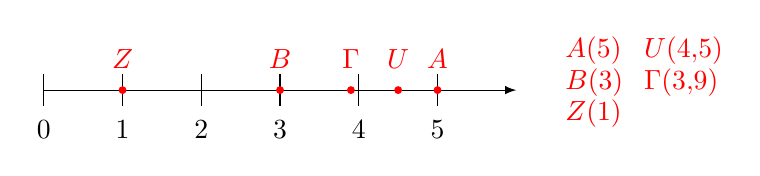
\begin{tikzpicture}[xscale=1]
    \draw[-latex] (0,0) -- (6,0);
    \foreach \x in {0,...,5} {
        \draw (\x, -0.2) -- +(0,0.4);
        \node at (\x, -0.5) {\( \x \)};
    };
    \foreach[count=\index from 0] \p/\x in {A/5, B/3, Z/1, U/4.5, \Gamma/3.9} {
        \fill[red] (\x,0) circle (0.05);
        \node[red] at (\x, 0.4) {\( \p \)};
        \node[red,anchor=west] at ({6.5+floor(\index /3)}, {0.5-0.4*mod(\index,3)}) {\( \p(\num{\x}) \)};
    }
\end{tikzpicture}
\end{document}